%
% teil3.tex -- Beispiel-File für Teil 3
%
% (c) 2020 Prof Dr Andreas Müller, Hochschule Rapperswil
%
% !TEX root = ../../buch.tex
% !TEX encoding = UTF-8
%
\subsection{Initialisierung
\label{genetic_algorithm:initialization}}
Der Startpunkt des genetischen Algorithmus ist die Initialisierung.
Dabei wird eine zufällige Population von möglichen Lösungen erstellt.
Diese wird als ein genetischer String dargestellt.

\begin{figure} [h]
	\centering
	
\includegraphics[width=0.8\textwidth]{
        papers/variationsprinzip_algorithmen/images/teil3/01_genetic_string.png
        }
	\caption{Beispiel eines möglichen genetischen Strings}
	\label{fig:possible_genetic_string}
\end{figure}

In jeder Position kann ein Gen aktiviert (1) oder deaktiviert (0) sein.
Diese Darstellung eignet sich jedoch nicht für das Travelling Salesman 
Problem (TSP), da eine Stadt nicht einfach ein- oder ausgeschaltet werden kann.
Auf die Wege ist es auch nicht anwendbar, das dann immer nur 1 Weg der vielen Wege 
aktiviert werden kann. Im TSP ist die Reihenfolge der Städte entscheidend. 
Daher wird die jeweilige Nummer der Stadt verwendet, wie im folgenden Bild 
\cite{cities_genetic_string} dargestellt:

\begin{figure} [h]
	\centering
	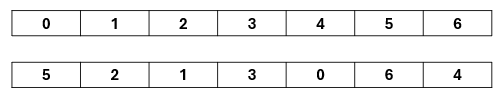
\includegraphics[width=0.8\textwidth]{
        papers/variationsprinzip_algorithmen/images/teil3/02_genetic_string_cities.png
        }
	\caption{Beispiel von Städten in einem genetischen String dargestellt}
	\label{fig:cities_genetic_string}
\end{figure}

Anstatt alle möglichen Lösungen zu erstellen, wird nur ein kleiner Teil 
(Population) zufällig generiert und weiter bearbeitet. Diese Taktik 
spart Zeit und Ressourcen.

Die zufällige Erzeugung der Anfangspopulation stellt ebenfalls eine Form 
der Variation dar. Sie sorgt dafür, dass die Suche nicht von einem begrenzten 
Bereich des Lösungsraums startet, sondern eine breite Palette von möglichen 
Lösungen berücksichtigt. Dabei werden jedoch keine Berechnungen durchgeführt, 
sondern zufällige Lösungen erstellt, in der Hoffnung, dass eine davon nahe 
an das Optimum herankommt.

